%%%%%%%%%%%%%%%%%%%%%%%%%%%%%%%%%%%%%%%%%%%%%%%%%%%%%%%%%%%%%%%%%%%%%%%%%%%%%%%
% Chapter 3: Procedimiento experimental 
%%%%%%%%%%%%%%%%%%%%%%%%%%%%%%%%%%%%%%%%%%%%%%%%%%%%%%%%%%%%%%%%%%%%%%%%%%%%%%%
%++++++++++++++++++++++++++++++++++++++++++++++++++++++++++++++++++++++++++++++
\section{Descripción de los experimentos}
\label{3:sec:1}
El experimento ha consistido en la implemenación en Python de algoritmos capaces de resolver el problema en cuestión. Para ello se ha creado una función cuya labor es calcular el seno dada cualquier x, otra que calcula las diferencias divididas a partir de una serie de nodos, una tercera que nos calcula el polinomio resultante que aproxima la función y por último una funcción de prueba donde se dan unos valores comprendidos en el intervalo de aproximacíon y compara su seno con el valor propuesto por nuestro polinomio.

%++++++++++++++++++++++++++++++++++++++++++++++++++++++++++++++++++++++++++++++
\section{Descripción del material}
\label{3:sec:2}
    Para la realización de este experimento el material necesario ha sido el siguiente:
 \begin{itemize}
  \item El ordenador usado en la realizacción de dicho experimento ha sido un portátil de la marca hp con un procesador Intel Atom{\tiny inside}. Este consta de 231,9 Gb de disco duro y 2 Gb de memoria RAM.
  \item El sistema operativo con el que hemos trabajado es una adaptación de la distribución de Linux \textit{kubuntu} a las necesidades en cuanto a Software de los miembros de la comunidad universitaria ULL: Bardinux \cite{url:bardinux}. 
 
  \begin{figure}[!h]
  \begin{center}
  
\includegraphics[scale=0.15]{images/bardinux.eps}
  \end{center}
  \caption{Logo Bardinux}
  \label{graph:1}
  \end{figure}
  \item También hemos hecho uso de materiales tales como calculadora, folio y lápiz, pues han habido cuestiones que han sido necesarias resolver a mano para la posterior implementación del código.
 \end{itemize}
 
%++++++++++++++++++++++++++++++++++++++++++++++++++++++++++++++++++++++++++++++
\section{Resultados obtenidos}
\label{3:sec:3}
Tras la implementación del código y la obtención del polinomio de aproximación hemos comprobado su precisión dando valores a las x y estos han sido resultados de algunos ejemplos:
\vspace{1.5 true cm}


\begin{figure}[!h]
\includegraphics[scale=0.38]{images/comprobacion.eps}
\caption{Consola}
\label{graph:2}
\end{figure}
%++++++++++++++++++++++++++++++++++++++++++++++++++++++++++++++++++++++++++++++
\section{Análisis de los resultados}
\label{3:sec:4}
A la hora de analizar la calidad de las aproximaciones dadas, se puede observar que, aunque buenas, estas no son del todo exactas. Desde un punto de vista teórico, si quisieramos unos mejores resultados en las aproximaciones, una solución efectiva sería seleccionar un mayor número de nodos. En nuestro caso el número de nodos en los que hemos dividido el intervalo $(0, \pi/2)$ es de 4: $(0, \pi/6, \pi/3, \pi/2)$; dejando entre cada uno de ellos un espacio equidistante.
Otro punto de vista a la hora de analizar los datos que hay que tener en cuenta es la calidad del material utilizado, en nuestro caso, las diferentes características de la máquina de cómputo mencionadas anteriormente.
\begin{figure}[H]
\begin{center}
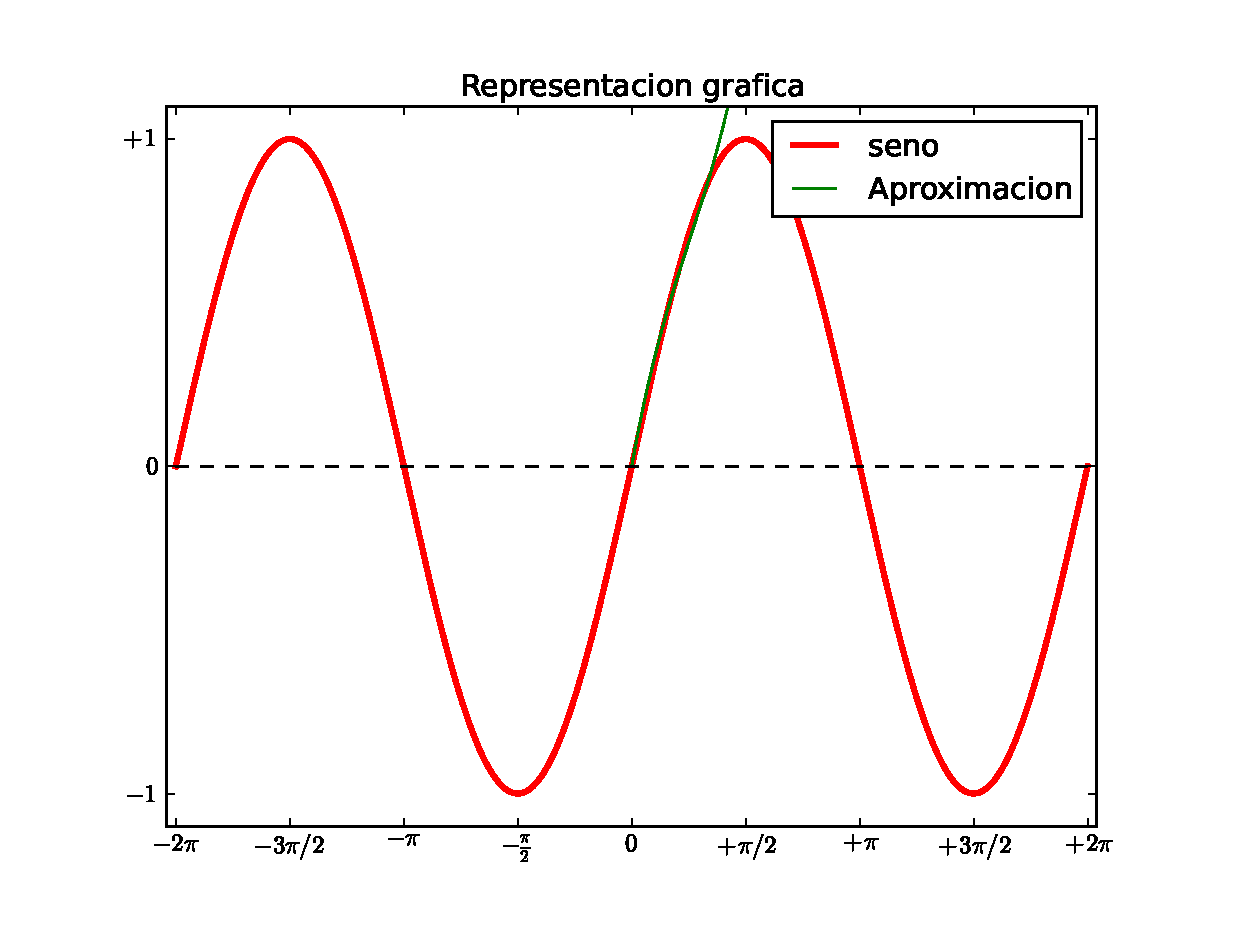
\includegraphics[scale=0.45]{images/representacionseno.eps}
\end{center}
\caption{Seno con Matplotlib}
\label{graph:4}
\end{figure}
